
\SC{I suggest you motivate this section by referencing Stephens et al. (2017), who did something similar.}

Once the polarization vector maps were created, the observed polarization morphologies were modelled using two geometric models. The models were created to reproduce the observed polarization morphologies, including azimuthal patterns (Figure \ref{fig: kataoka_polarization_morphologies}a), polarization vectors that uniformly align with the minor axis (Figure \ref{fig: kataoka_polarization_morphologies}b), and intermediate morphologies. Since dust self-scattering is expected to produce a uniform pattern, the model allows us to identify the regions of the disk where scattering-induced polarization may dominate. 

A more physical model could include radiative transfer. The goal here is to identify the regions of the disk where the signatures of each polarization mechanism dominate, rather than to model the physical mechanisms that produce the observed patterns. The two geometric models are described below.

\SC{comment}


\subsection{Goodness of Fit}

To determine how well a geometric model reproduced the polarization observations, a chi-squared value was calculated. First, the difference between the observed and model-predicted polarization angle needed to be calculated carefully. Polarization angles can range from 0--180\degg because polarization measures orientation, rather than direction, meaning that angles that are 180\degg apart have the same polarization vector orientation. As a result, two polarization angles that are physically very similar can have a large numerical difference. For example, polarization angles of 1\degg and 179\degg only differ by 2\deggNS, but directly taking their difference would give 178\deggNS. To account for this, the angular difference is defined by the minimum angular separation between the two angles:
\begin{equation}
    \Delta \theta = \text{min}(|\theta_{\text{obs}} - \theta_{\text{model}}|, 180\deggEQ - |\theta_{\text{obs}} - \theta_{\text{model}}|),
    \label{eq: minimum_separation}
\end{equation}

\noindent where $\theta_{\text{obs}}$ is the observed polarization angle and $\theta_{\text{model}}$ is the polarization angle predicted by either the ratio or Gaussian model. The angular differences were then used to calculate the chi-squared value:
\begin{equation}
    \chi^2 = \sum \left(\frac{\Delta \theta_i}{\sigma_\theta}\right)^2,
    \label{eq: chi_sq}
\end{equation}
\noindent where the angular distance is summed over all sampled polarization vectors. 

The value of $\chi^2$ was then converted to reduced chi-squared by:
\begin{equation}
    \chi^2_{reduced} = \frac{1}{n-k} \times \chi^2,
    \label{eq: chi_sq_reduced}
\end{equation}
\noindent where $n$ is the number of sampled polarization vectors and $k$ is the degrees of freedom. For the ratio model, there is one degree of freedom, and for the Gaussian method, there are three ($\phi$, $b$, and $a$). 

% ----------------------------------------------------------
\subsection{Ratio Model}
% ----------------------------------------------------------



The first geometric model tested is the \emph{ratio model}. The main idea behind this model is to reproduce the observed polarization morphologies, ranging from purely aligned with the minor axis of the disk to purely azimuthal, along with intermediate cases. This was achieved by creating a grid of models weighted between these two extreme cases. 

The first extreme case is a 100\% uniform pattern, where every vector is aligned with the minor axis of the disk (90\degg from the disk position angle, Table \ref{tab: source_info}).  This is shown in the left panel of Figure \ref{fig: RatioExamples}. The second extreme case is a 100\% azimuthal pattern, where the polarization vectors follow a circular pattern around the centre of the disk. The centre point of the disk at each wavelength can be found in Table \ref{tab: source_info}. For each pixel $(x, y)$, the offset from the disk centre $(x_c, y_c)$ is calculated as:
\begin{equation}
\begin{aligned}
    \delta x &= x - x_c, \\
    \delta y &= y - y_c.
\end{aligned}
% \label{eq: vectors}
\end{equation}


\noindent These offsets are then used to calculate the azimuthal polarization angle using \texttt{numpy.arctan2}. This is shown in the right panel of Figure \ref{fig: RatioExamples}.



To create the intermediate cases, models were generated in steps of 10\% and are denoted as $N \uni + (100 - N) \azi$, where $N = 0, 10 \ldots, 100$. Here, Uni and Azi represent the pure uniform and pure azimuthal cases, respectively, and $N$ gives the percentage contribution of the uniform case. 

Since the polarization angles cannot be directly combined, the \SQ and \SU for the extreme cases ($100\uni+0\azi$ and $0\uni+100\azi$) were calculated from the polarization angle grids using:

\begin{equation}
\begin{aligned}
Q_{\text{Uni}} &= \rho I \cos(2\theta_{\text{Uni}}) \text{ and }
Q_\text{Azi} = \rho I \cos(2\theta_\text{Azi}),
     \\
U_{\text{Uni}} &=  \rho I \sin(2\theta_{\text{Uni}}) , \text{ and }
U_\text{Azi} =  \rho I \sin(2\theta_\text{Azi}) 
\end{aligned}
% \label{eq:50U50A}
\end{equation}
\noindent following \cite{Montier}, where $\rho$ is the average polarization fraction over the centre and edges, which fixed at 2\%. This value is expected to be reasonable for the uniform polarization morphology, but the polarization fraction may differ for the azimuthal morphology, potentially biasing the azimuthal case low.

%This is consistent with values of 0.02-0.03 from \cite{Kataoka_2017}, 



The intermediate \SQ and $U$ maps were then obtained by combining the two extreme models using:
\begin{equation}
\begin{aligned}
Q_{N}
    &= \frac{N}{100}\,Q_{\text{Uni}}
     + \frac{100 -N}{100}\,Q_{\text{Uni}}, \\
U_{N}
    &= \frac{N}{100}\,U_{\text{Uni}}
     + \frac{100 -N}{100}\,U_{\text{Azi}}.
\end{aligned}
% \label{eq:50U50A}
\end{equation}

\noindent The resulting $Q_N$ and $U_N$ model maps were used to calculate the model polarization angle at each pixel using Equation \ref{eq: PA}. The polarization vectors were generated using the methods in Chapter \ref{sec: chap4_polarization_vectors}. This process was repeated for each ratio combination. For example, $N=50$ corresponds to the $50\uni+50\azi$ model, shown in the middle panel of Figure \ref{fig: RatioExamples}.





\begin{figure}[htbp]
  \centering
  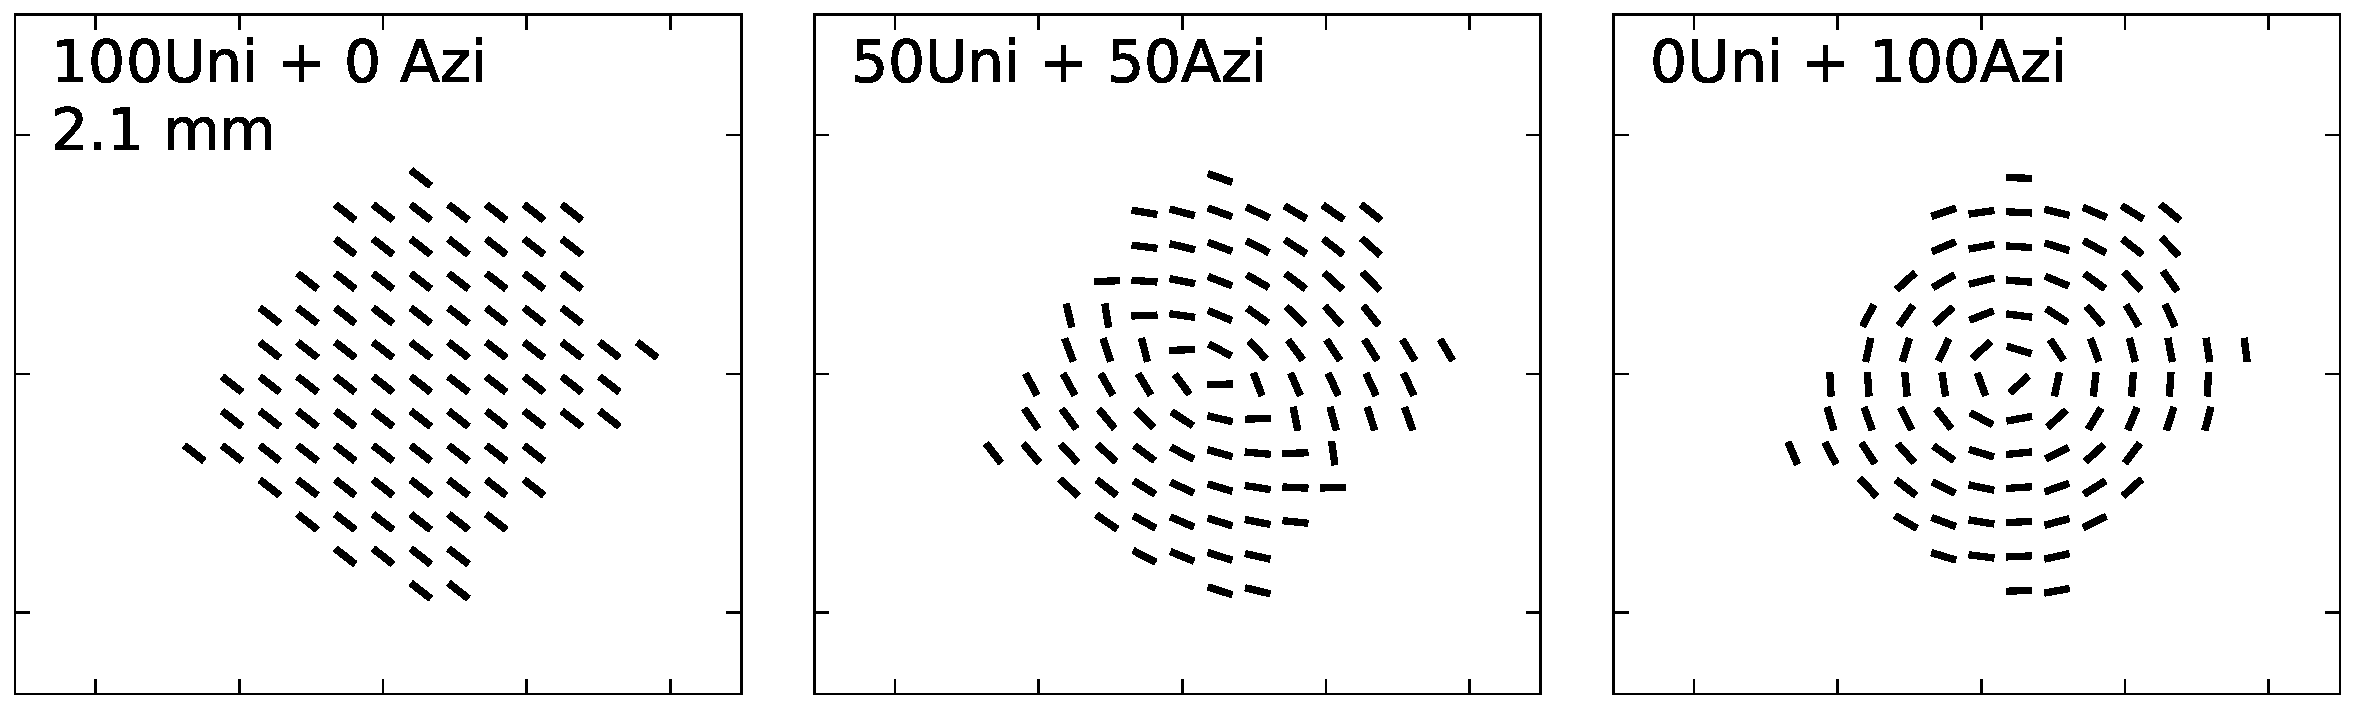
\includegraphics[width=0.99\textwidth]{WRITEUP_AND_IMAGES/IMAGES/WRITEUP/Ratio/RatioExamplesTest_Band4_NoAxes.pdf}
  \caption[Example of the $N = 100, N=50$ and $N = 0$ cases of the ratio model.]{Example of the $N = 100, N=50$ and $N = 0$ cases of the ratio model for \bfourNS.}
  \label{fig: RatioExamples}
\end{figure}





For the ratio models, Table \ref{tab:ratio_model_chi2} presents the \chired values calculated for each test with the best-fit value shown in bold.  Figure \ref{fig: RatioBestGrid} shows the best-fit model with the observed vectors in black and the model vectors in red.


Taking \bfive as an outlier (see Chapter \ref{sec: discussion_band5_data_issues}), the best-fit ratio models show that, as wavelength decreases, the observations are better matched with a higher uniform contribution. This result is consistent with the observations discussed in Chapter \ref{sec: c4_polarization_maps}, which show a greater uniform contribution with decreasing wavelength. 






% This was updated to Band 5 robust = -1 on July 18th
% These numbers might need to be changed if we change how we calculate chi^2
% This is Band 4 nterms2, Band 7 nterms 2.
\begin{table}[h!]
\centering
\caption[Ratio model fitting results.]{Ratio model fitting results for each wavelength, with goodness-of-fit quantified by $\chi^2_{reduced}$. Best fits are shown in bold. }
\begin{tabular}{lcccc}
\toprule
\textbf{Ratio Model} & \textbf{\bfour} & \textbf{\bfive} & \textbf{\bsix} & \textbf{\bseven} \\
\midrule
100Uni + 0Azi
& 181.67 % Band 4 
& \textbf{22.58} % Band 5 
& 37.39 % Band 6  
& \textbf{79.12} \\


90Uni + 10Azi
& 171.40 % Band 4
& 24.22 % Band 5  
& 33.93 % Band 6  
& 88.59 \\

80Uni + 20Azi
& 158.01 % Band 4 
& 27.77 % Band 5  
& \textbf{33.36} % Band 6  
& 108.65 \\

70Uni + 30Azi
& 140.74 % Band 4 
& 34.28 % Band 5  
& 37.99 % Band 6 
& 144.84 \\

60Uni + 40Azi
& 116.11 % Band 4 
& 45.10 % Band 5
& 51.96 % Band 6 
& 206.76 \\

50Uni + 50 Azi
& \textbf{88.21} % Band 4 
& 63.81 % Band 5  
& 84.48 % Band 6  
& 322.01 \\

40Uni + 60Azi
& 124.99 % Band 4 
& 91.17 % Band 5  
& 140.41 % Band 6  
& 498.43 \\

30Uni + 70 Azi
& 131.03 % Band 4 
& 116.35 % Band 5
& 191.20 
& 647.50 \\

20Uni + 80Azi
& 133.70 % Band 4 
& 138.36 % Band 5  
& 233.90 % Band 6  
& 776.00 \\

10Uni + 90Azi
& 136.42 % Band 4
& 157.27 % Band 5  
& 270.41 % Band 6 
& 886.40 \\

0Uni + 100Azi
& 139.41
& 173.26
& 302.34 
& 979.97 \\
\bottomrule
\end{tabular}
% \begin{tablenotes}
% \footnotesize
% \item \textbf{Note:} Values of . 
% \end{tablenotes}
\label{tab:ratio_model_chi2}
\end{table}





% PLOTS
% ----------------------------------------
% ----------------------------------------
% \begin{figure*}[h]
%   \centering

%   % Row 1
%   \begin{minipage}{0.48\textwidth}
%     \centering
%     
\includegraphics[width=\linewidth]{IMAGES/WRITEUP/Ratio/IRS63_best_ratio_BAND4.pdf}
%     \textbf{(a) Band 4}
%   \end{minipage}
%   \hfill
%   \begin{minipage}{0.48\textwidth}
%     \centering
%     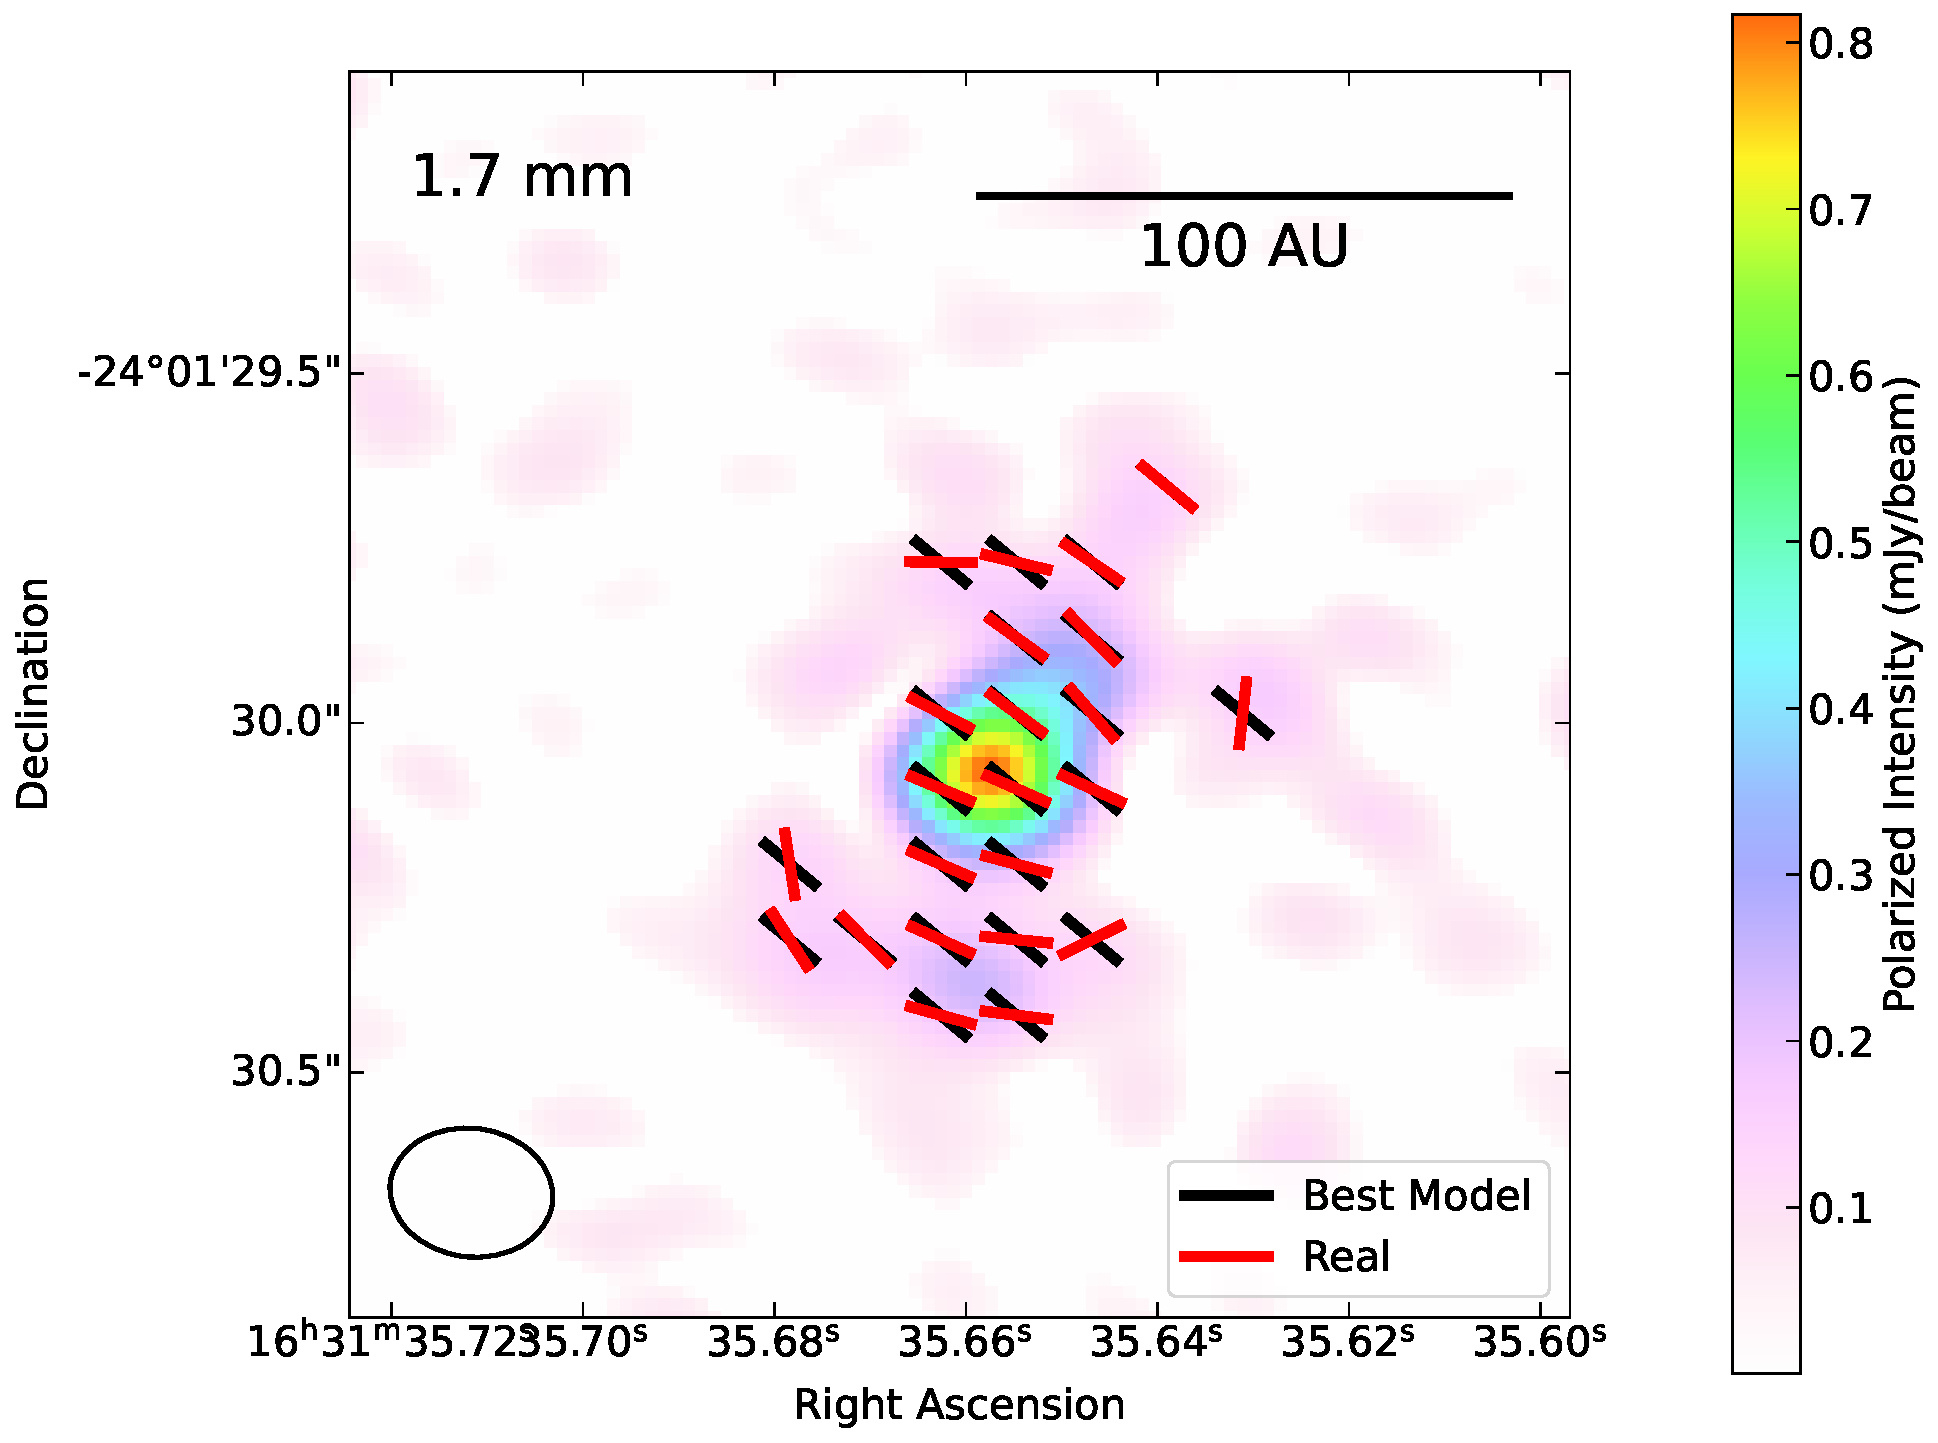
\includegraphics[width=\linewidth]{IMAGES/WRITEUP/Ratio/IRS63_best_ratio_BAND5_robust_minus1.pdf}
%     \textbf{(b) Band 5}
%   \end{minipage}

%   \vspace{0.5cm}

%   % Row 2
%   \begin{minipage}{0.48\textwidth}
%     \centering
%     \includegraphics[width=\linewidth]{WRITEUP_AND_IMAGES/
%   \end{minipage}
%   \hfill
%   \begin{minipage}{0.48\textwidth}
%     \centering
%     
\includegraphics[width=\linewidth]{IMAGES/WRITEUP/Ratio/IRS63_best_ratio_BAND7.pdf}
%     \textbf{(d) Band 7}
%   \end{minipage}

%   \caption{
%   \add{caption, make this a grid} \note{Change to $\Delta\alpha$ and $\Delta \delta$ if we chose to do that for other plots.} \note{Update to band 5 robust -1}
%   }

%   \label{fig:best-ratio-models}
% \end{figure*}
% ----------------------------------------
% ----------------------------------------





\begin{figure}[htbp]
  \centering
  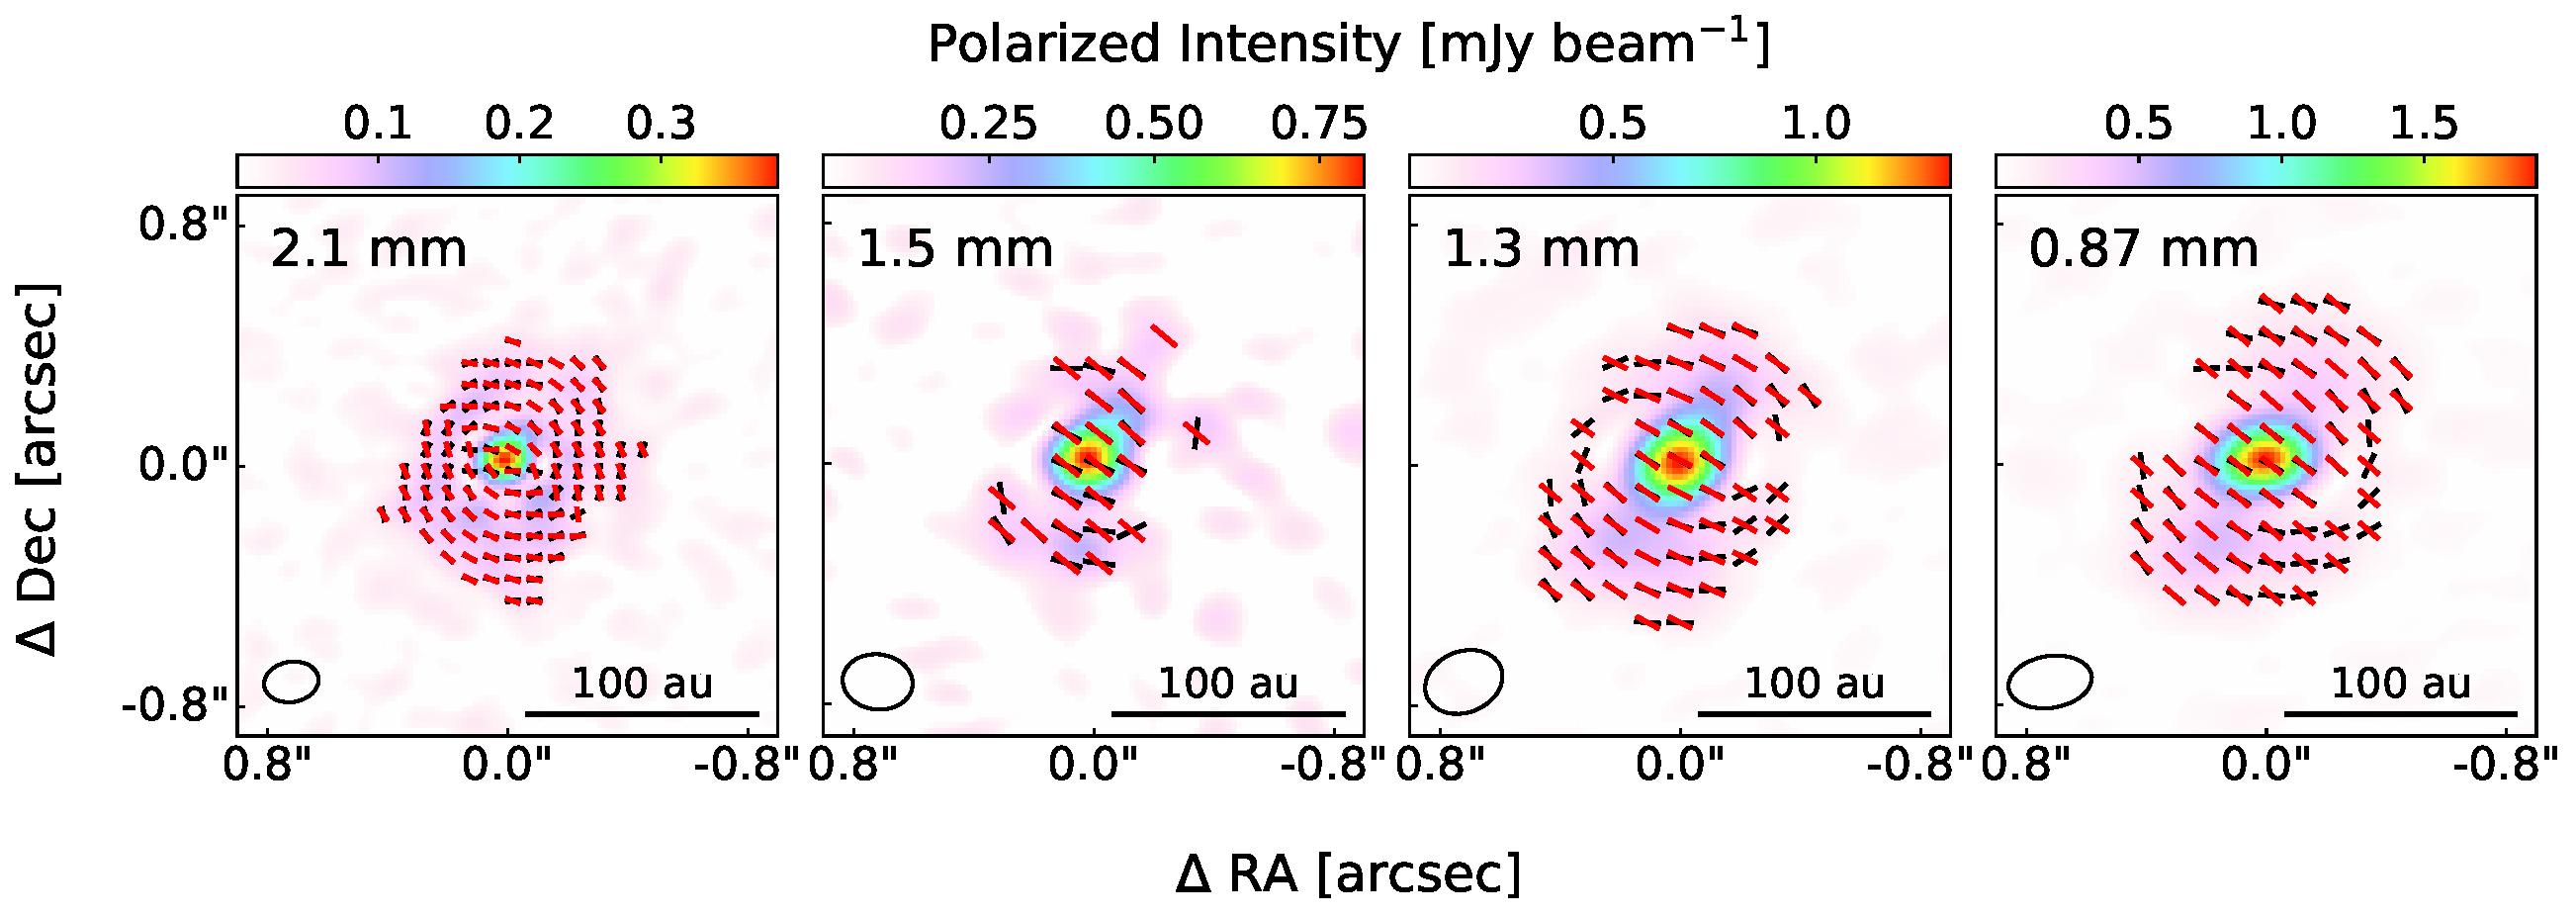
\includegraphics[width=0.99\textwidth]{WRITEUP_AND_IMAGES/IMAGES/WRITEUP/Ratio/Best_grid_Delta.pdf}
  \caption[Figure \ref{fig: StokesI_POLI_grid}, with the polarization vectors from the best-fit ratio model.]{Figure \ref{fig: StokesI_POLI_grid}, overplotted with the polarization vectors in red from the best-fit ratio model at each wavelength. The corresponding best-fit ratio models are listed in Table \ref{tab:ratio_model_chi2}.  }
  \label{fig: RatioBestGrid}
\end{figure}






% ----------------------------------------------------------
\subsection{Gaussian Model}
% ----------------------------------------------------------


The second geometric model tested is the \emph{Gaussian model}. The aim of this model was to reproduce a polarization morphology that transitions from being aligned with the minor axis of the disk at the centre to becoming more azimuthal towards the outer parts of the disk. This is based on the expectation that the emission from the inner region is optically thick \citep{Kataoka_2015}, with optical thickness decreasing towards the outer edge of the disk. 


To achieve this, we used a rotated 2-dimensional flat-topped Gaussian model with three free parameters: $\phi$, $a$ and $b$. The Gaussian was calculated using the equation :
\begin{equation}
W_{\text{Uniform}} =  I_0 
\exp\left[-\half \left(\left|\frac{X_{M}}{\sigma_M}\right|^\phi + \left|\frac{Y_{m}}{ \sigma_m}\right|^\phi\right)\right],
    \label{eq: gaussian_eq}
\end{equation}
\noindent where $I_0$, the peak value, was calculated using the equation:
\begin{equation}
    I_0 = \frac{1} {\sigma_m \sigma_M \sqrt{2\pi}}.
    \label{eq: Gaussian_model_I0}
\end{equation}

\noindent In Equation \ref{eq: gaussian_eq}, $\phi=2$ corresponds to a standard 2D Gaussian, while $\phi>2$ produces a flat-topped Gaussian. Table \ref{tab: gaussian_model_info} lists the parameters and the ranges we tested. The tested values of $a$ and $b$ control the widths of the Gaussian model (major and minor axes of the Gaussian, respectively), with each treated as the FWHM and converted to standard deviations using Equation \ref{eq: FWHM_to_sigma}. Additionally, a condition of $b$ $\leqq $ $a$ was required to ensure the minor axis was smaller than the major axis. 


% \begin{equation}
% f(x) = A \exp{\left(-\left(\frac{(x-x_0)^2}{2\signa_X^2}\right)^P\right)}
%     \label{eq: super-Gaussian}
% \end{equation}
% \question{do I need to cite this? I got it from Wikipedia.}


\begin{table}[h!]
\centering
\caption{Summary of parameters and tested values in the Gaussian model.  }
\begin{tabular}{lll}
\toprule
\textbf{Property} &
\textbf{Meaning} &
\textbf{Tested Values}  \\
\midrule

$\phi$
& super-Gaussian exponent
& 2, 3, 4, 5, 6, 7\\


$a$ (pixels)
& major axis of Gaussian
& 10, 20, 30, 40, 50\\

$b$ (pixels)
& minor axis of Gaussian
& 10, 20, 30, 40, 50\\

\bottomrule
\end{tabular}
\label{tab: gaussian_model_info}
\end{table}


The Gaussian was rotated to align with the major axis of the disk, using the position angle of the disk (\PAns) given in Table \ref{tab: source_info}. The coordinates ($x, y$) were shifted with respect to the centre of the disk ($x_c, y_c$) and then rotated:
\begin{equation}
\begin{pmatrix}
X_M \\
Y_m
\end{pmatrix}
=
\begin{pmatrix}
\cos(\PAeq) & -\sin(\PAeq) \\
\sin(\PAeq) & \cos(\PAeq)
\end{pmatrix}
\begin{pmatrix}
x - x_c \\
y - y_c
\end{pmatrix}.
\label{eq:rotated_coordinates}
\end{equation}





\noindent The Gaussian was normalized to a maximum of 1 so that it could be used as a pixel weight. Equation \ref{eq: gaussian_eq} creates a map that specifies the weights for the Uniform polarization region of the disk, where the weight is 1 at the centre and drops to zero with radius.  We use 1 - \Wuni to give the weight for the azimuthal polarization morphology. These two maps act as our weights, rather than a constant like in the ratio model. 


The weighted \SQ and $U$ were calculated by:
\begin{equation}
\begin{aligned}
Q_{\text{Gaussian}}
    &= \WuniEQ \,Q_{\text{Uni}}
     + (1 - \WuniEQ)\,Q_{\text{Azi}}, \\
U_{\text{Gaussian}}
    &= \WuniEQ\,U_{\text{Uni}}
     + (1 - \WuniEQ)\,U_{\text{Azi}},
\end{aligned}
% \label{eq:50U50A}
\end{equation}

\noindent As in the ratio model, the maps of $Q_{\text{Gaussian}}$ and $U_{\text{Gaussian}}$ were used to calculate the position angle (Equation \ref{eq: PA}). Figure \ref{fig: Methods/GaussianExamples} shows two example Gaussian weight maps with polarization vectors overlaid.  The values of $\phi$, $a$, and $b$ are given in the lower-left corner.  The vector sampling is selected to match the \bfour data.


\begin{figure}[htbp]
  \centering
  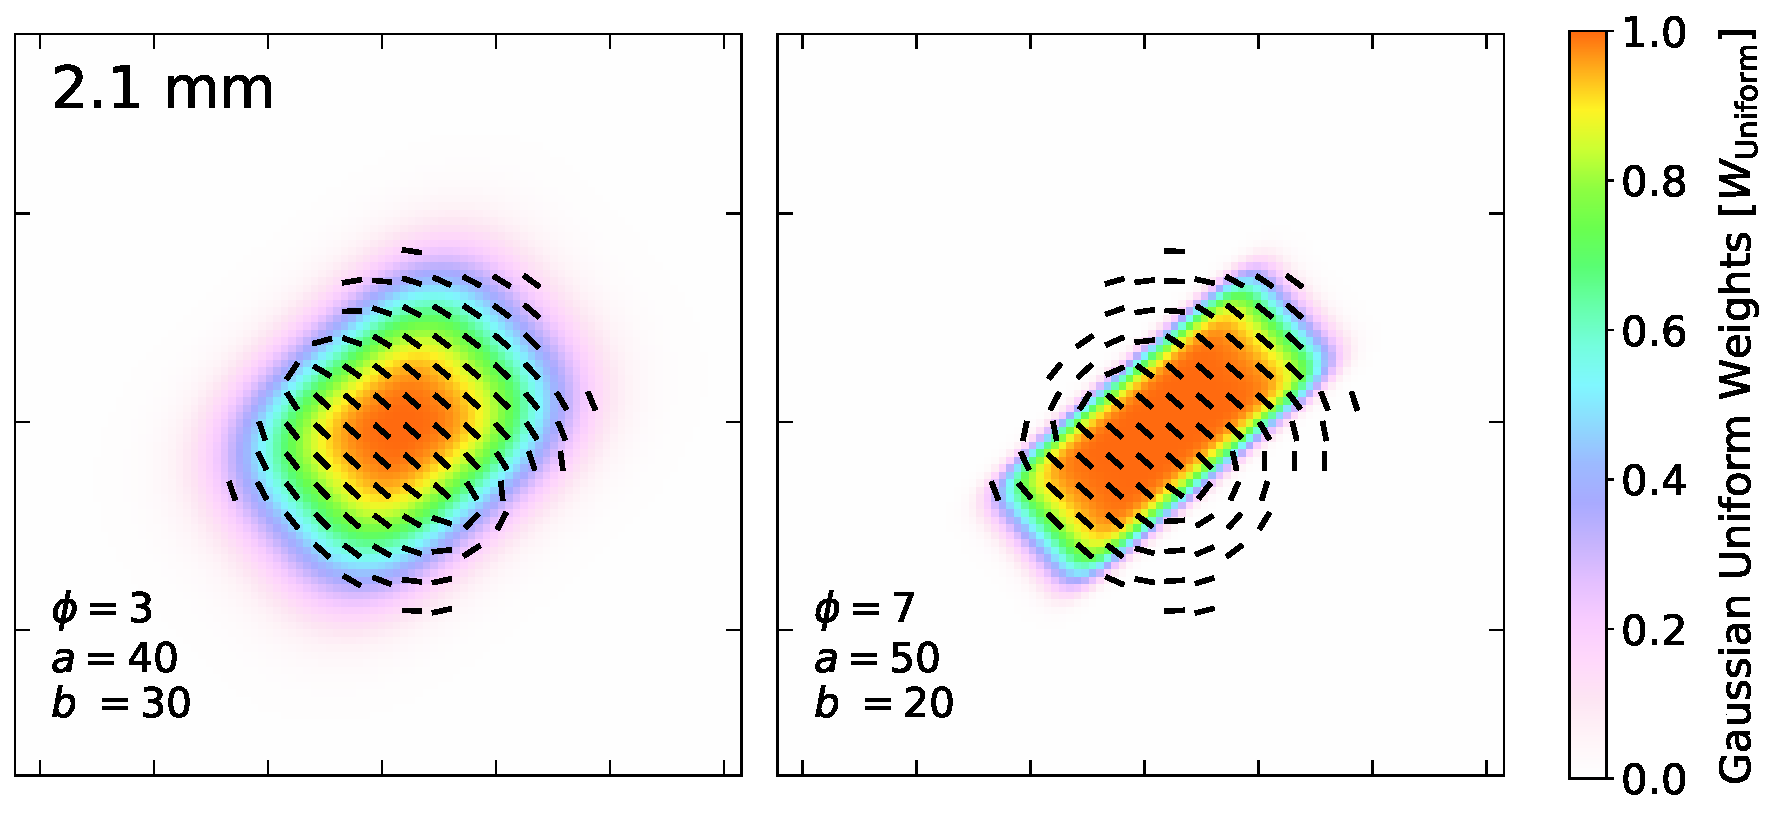
\includegraphics[width=0.8\textwidth]{WRITEUP_AND_IMAGES/IMAGES/WRITEUP/Gaussian/CustomExamples_B4.pdf}
  \caption{Two examples of the Gaussian weights for selected values of $\phi$, $a$ and $b$.}
  \label{fig: Methods/GaussianExamples}
\end{figure}





% ----------------------------------------------------------




For the Gaussian model, Table \ref{tab:gaussian_top5} presents the five best-fitting cases (out of 150 tested) with the best-fit model highlighted in bold.  Figure \ref{fig: GaussianBestGrid} compares the observed and model vectors for the best-fit models at each wavelength. 




\begin{figure}[htbp]
  \centering
  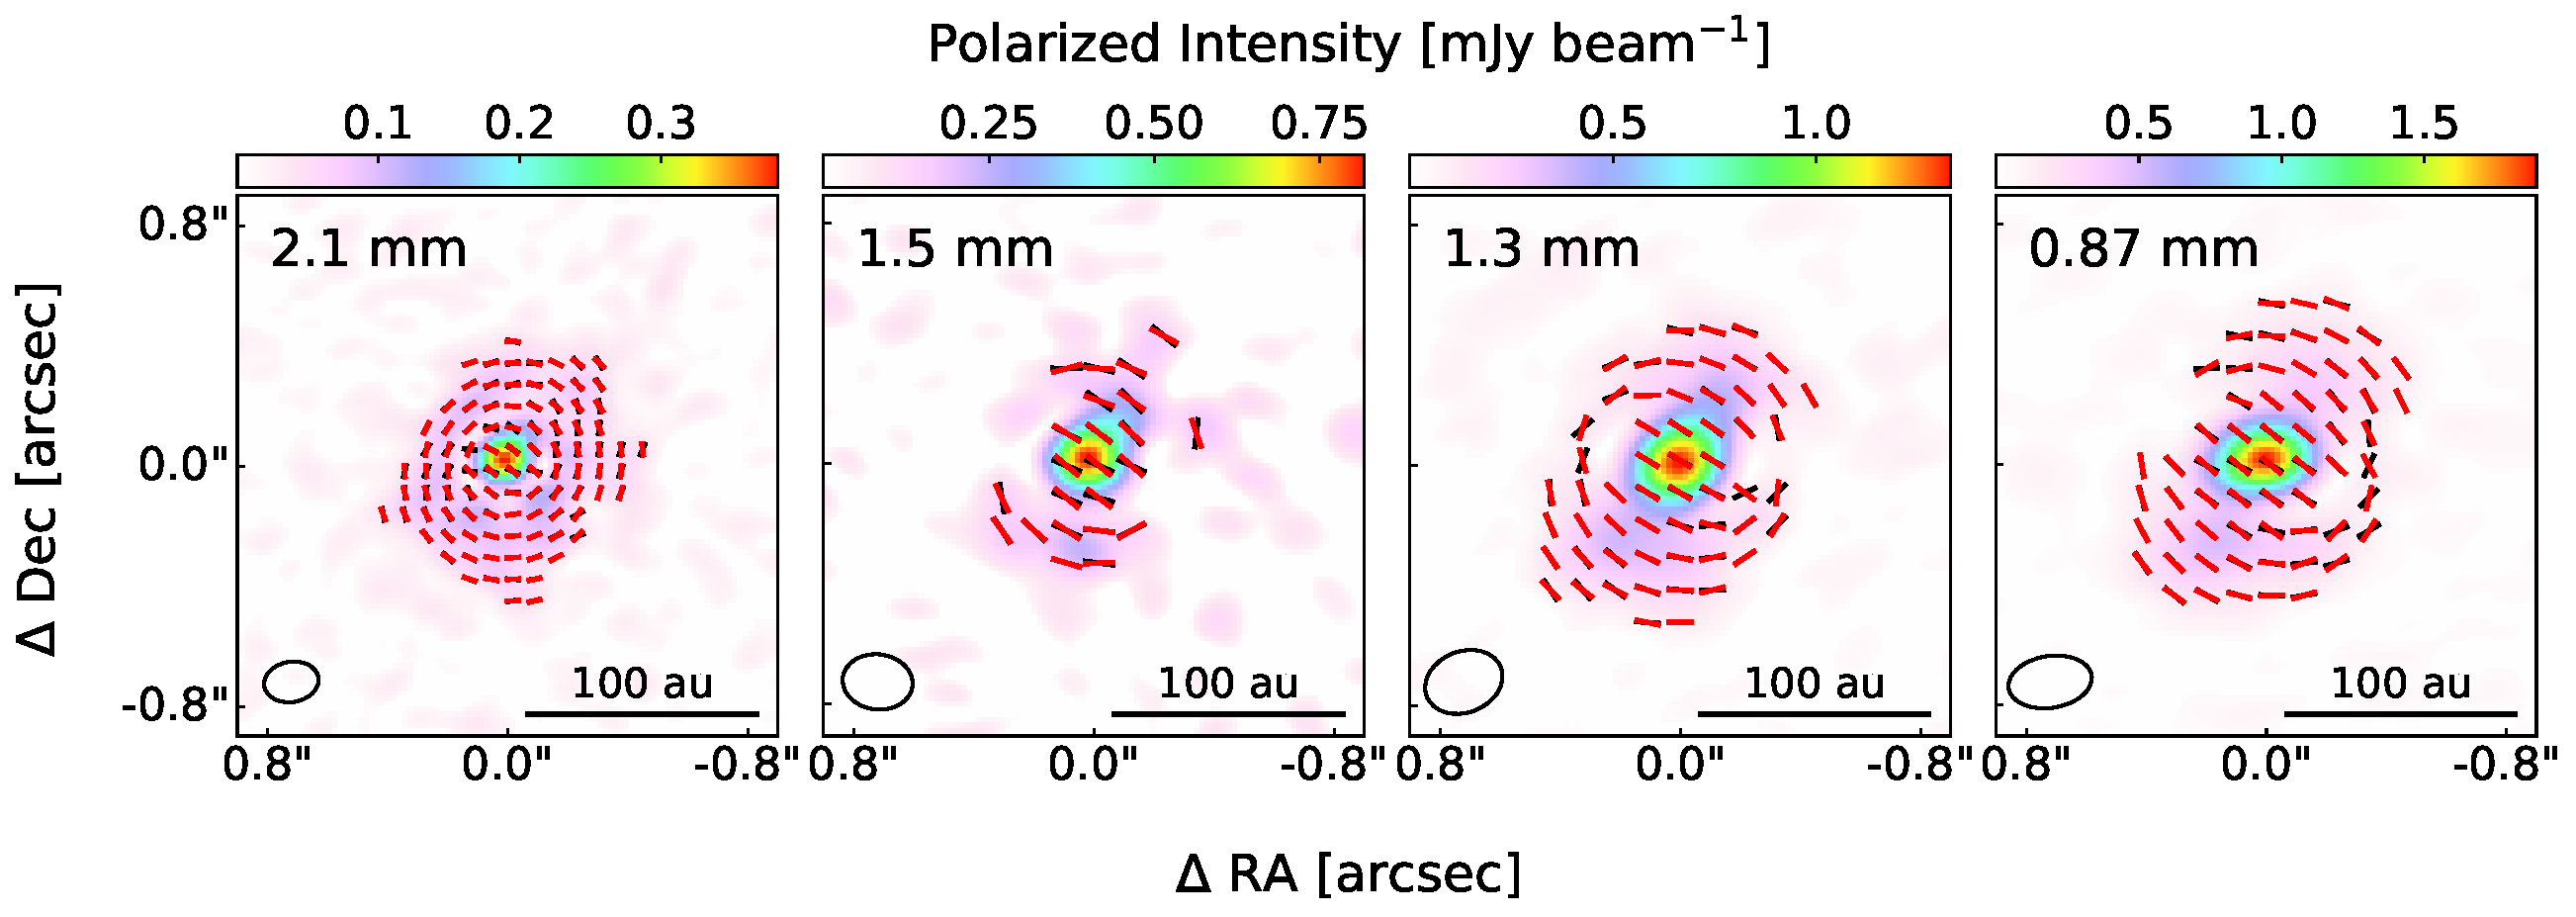
\includegraphics[width=0.99\textwidth]{WRITEUP_AND_IMAGES/IMAGES/WRITEUP/Gaussian/Best_grid_Delta.pdf}
  \caption{Same as Figure \ref{fig: RatioBestGrid}, but for the best-fit Gaussian models. The corresponding best-fit Gaussian models are listed Table \ref{tab:gaussian_top5}.}
  \label{fig: GaussianBestGrid}
\end{figure}





% This was updated to Band 5 robust = -1 on July 18th
% Needs updating if we change how we calculate chi-squared
% Band 4 and Band 7 nterms 2

\begin{table}[h!]
\centering
\caption{Top give Gaussian model fits at each wavelength, sorted by $\chi^2_{reduced}$. The best fit at each wavelength is shown in bold.}
\begin{tabular}{c ccc c}
\toprule
\textbf{Wavelength} & $\boldsymbol{\phi}$ & $\boldsymbol{a}$ & $\boldsymbol{b}$ &  $\boldsymbol{\chi^2}$ \\
\midrule

\textbf{\bfour} 
& \textbf{7} & \textbf{20} & \textbf{10} & \textbf{26.70} \\
 & 6 & 20 & 10 & 26.79 \\
 & 5 & 20 & 10 & 26.95 \\
 & 4 & 20 & 10 & 27.30 \\
 & 3 & 20 & 10 & 28.04 \\

\midrule

\textbf{\bfive} 
& \textbf{4} & \textbf{30} & \textbf{20} & \textbf{13.88} \\
 & 5 & 30 & 20 & 13.92 \\
 & 6 & 30 & 20 & 14.09 \\
 & 3 & 30 & 20 & 14.16 \\
 & 7 & 30 & 20 & 14.30 \\

\midrule

\textbf{\bsix} 
& \textbf{4} & \textbf{30} & \textbf{30} & \textbf{8.08} \\
 & 5 & 30 & 30 & 8.09 \\
 & 6 & 30 & 30 & 8.19 \\
 & 7 & 30 & 30 & 8.33 \\
 & 3 & 30 & 30 & 8.41 \\

\midrule

\textbf{\bseven} 
& \textbf{6} & \textbf{40} & \textbf{30} & \textbf{38.56} \\
 & 5 & 40 & 30 & 38.59 \\
 & 7 & 40 & 30 & 38.69 \\
 & 6 & 30 & 30 & 38.86 \\
 & 7 & 30 & 30 & 38.88 \\

\bottomrule
\end{tabular}
\label{tab:gaussian_top5}
\end{table}



  


From the results in Table \ref{tab:gaussian_top5}, the values of $a$ and $b$ are consistent among the top five models at each wavelength, but the values differ between wavelengths. This indicates that, within each wavelength, these values provide a good fit among the tested values. For simplicity, the area of the Gaussian is defined as:
\begin{equation}
A = a \cdot b.
    \label{eq: GaussianArea}
\end{equation}
\noindent A larger value of $A$ corresponds to a larger area of uniform morphology. For\bfourNS, \bfiveNS, \bsiNS, and \bsevenNS the corresponding areas are 200, 600, 900, 1200 pixels$^2$, respectively. The increase in area as wavelength decreases indicates the uniform morphology contributes over a larger region of the disk at shorter wavelengths. This can be seen in Figure \ref{fig: gaussian_best_map_w_uniform}, showing the Gaussian shape ($W_{\text{Uniform}}$) for the best-fit model at each wavelength.


\begin{figure}[htbp]
  \centering
  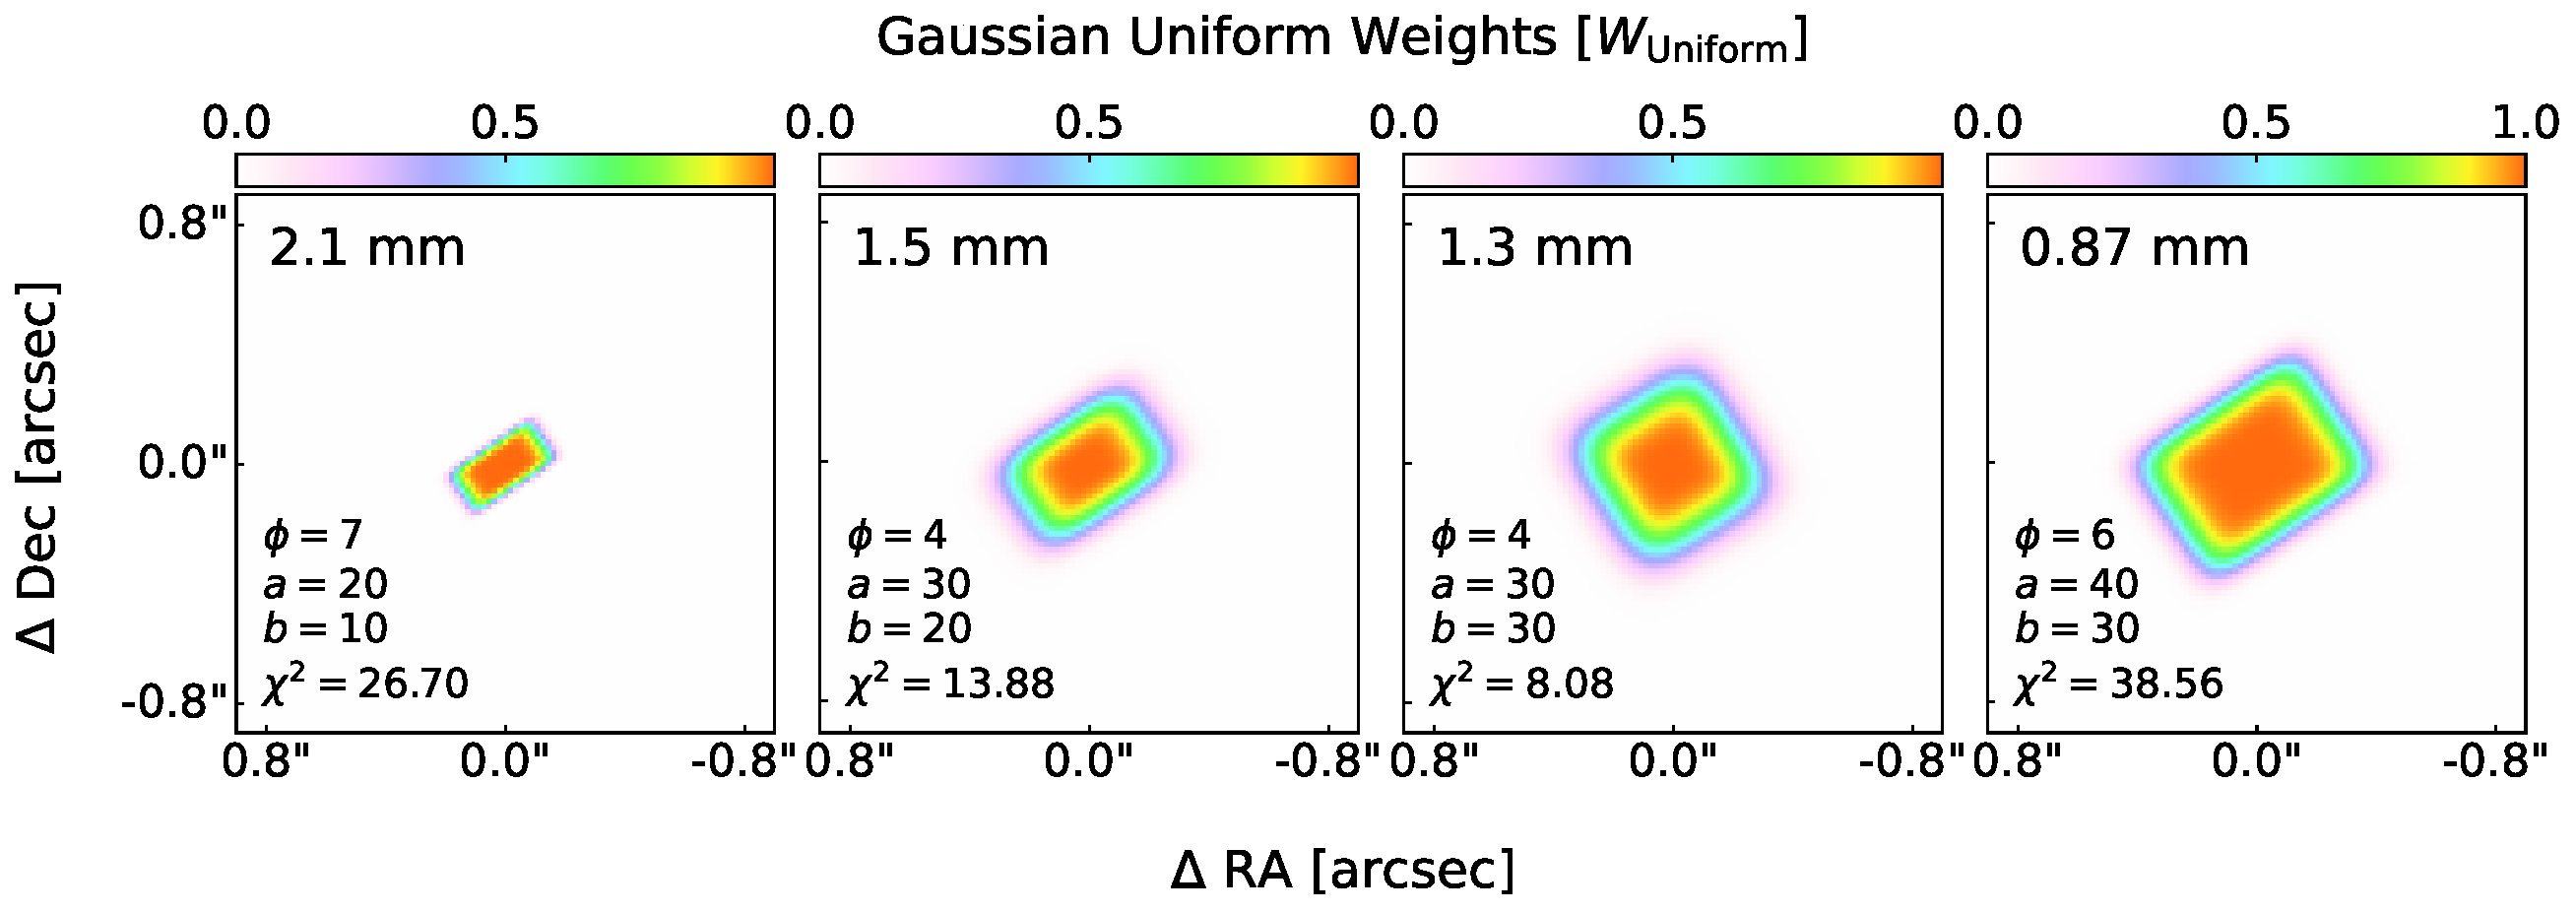
\includegraphics[width=0.99\textwidth]{WRITEUP_AND_IMAGES/IMAGES/WRITEUP/Gaussian/Best_grid_Delta_map.pdf}
  \caption{Maps of the Gaussian uniform weights $W_{\text{uniform}}$ (Equation \ref{eq: gaussian_eq}) for the best-fit Gaussian model for each wavelength, corresponding vector pattern shown in Figure \ref{fig: GaussianBestGrid}. }
  \label{fig: gaussian_best_map_w_uniform}
\end{figure}




The parameter $\Phi$ changes the flatness of the Gaussian, the higher the $\Phi$ value the flatter the Gaussian, transitioning from uniform to azimuthal morphology faster (see Figure \ref{fig: Methods/GaussianExamples}). In the best-fit model at each wavelength, $\Phi$ is greater than 2, producing a flat-topped Gaussian rather than a standard Gaussian. This can also be seen in Figure \ref{fig: gaussian_best_map_w_uniform}, which shows that the area of uniform alignment increases as wavelength decreases. This indicates that uniform alignment, which is consistent with dust self-scattering, contributes more at shorter wavelengths, which is what we expect from Chapter \ref{sec: c4_polarization_maps} and the results from the ratio model. 













% PLOTS
% ----------------------------------------
% ----------------------------------------
% \begin{figure*}[h]
%   \centering

%   % Row 1
%   \begin{minipage}{0.48\textwidth}
%     \centering
%     
\includegraphics[width=\linewidth]{IMAGES/WRITEUP/Gaussian/IRS63_best_gaussian_BAND4.pdf}
%     \textbf{(a) Band 4}
%   \end{minipage}
%   \hfill
%   \begin{minipage}{0.48\textwidth}
%     \centering
%     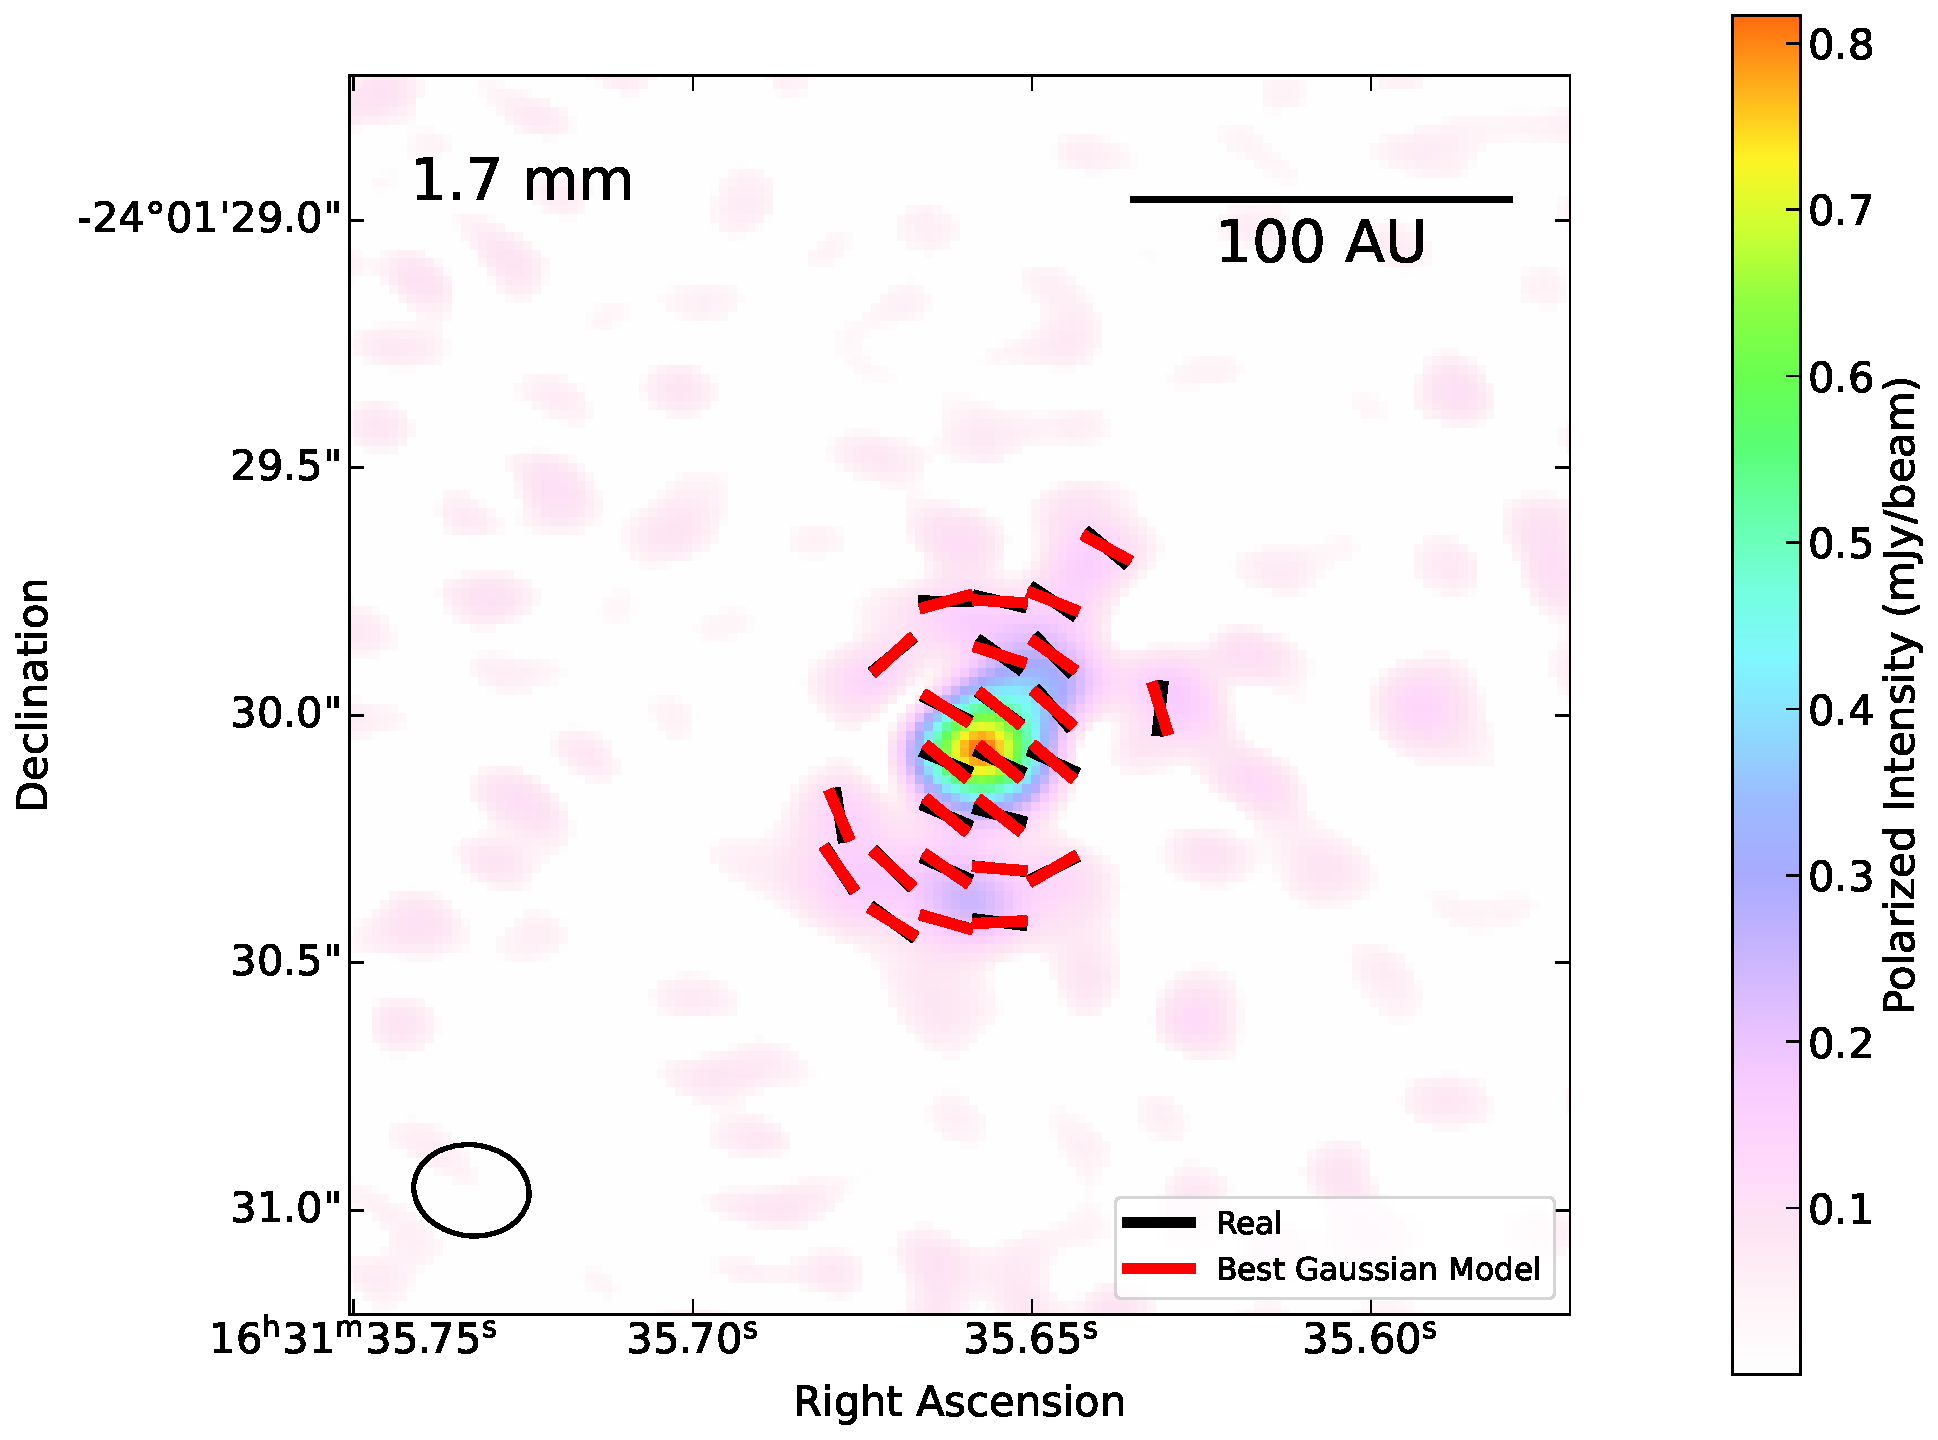
\includegraphics[width=\linewidth]{IMAGES/WRITEUP/Gaussian/IRS63_best_gaussian_BAND5_robust_minus1}
%     \textbf{(b) Band 5}
%   \end{minipage}

%   \vspace{0.5cm}

%   % Row 2
%   \begin{minipage}{0.48\textwidth}
%     \centering
%     
\includegraphics[width=\linewidth]{IMAGES/WRITEUP/Gaussian/IRS63_best_gaussian_BAND6.pdf}
%     \textbf{(c) Band 6}
%   \end{minipage}
%   \hfill
%   \begin{minipage}{0.48\textwidth}
%     \centering
%     
\includegraphics[width=\linewidth]{IMAGES/WRITEUP/Gaussian/IRS63_best_gaussian_BAND7.pdf}
%     \textbf{(d) Band 7}
%   \end{minipage}

%   \caption{
%   \add{caption, make this a grid} \note{Change to $\Delta\alpha$ and $\Delta \delta$ if we chose to do that for other plots.} \note{Update to band 5 robust -1}
%   }

%   \label{fig:best-gaussian-models}
% \end{figure*}
% ----------------------------------------
% ----------------------------------------







% ----------------------------------------------------------




% ----------------------------------------------------------
\subsection{Comparison of Geometric Models}
% ----------------------------------------------------------

% ----------------------------------------------------------


